\state{Exchange}{
	Consider single-particle wavefunctions on two neighboring identical atoms $\psiA, \psiB$, which may be assumed real.  These are to be used as the basis for a two-electron state.  Show that the charge density in a singlet (triplet) state made out of the two orbitals is given by
	\eq{
		\rhor = \abs{\psiAr}^2 + \abs{\psiBr}^2 \pm 2 \bkpsiAB \psiAr \psiBr.
	}
	Explain why the singlet state will usually be lower in energy.
}

\sol{
	The charge density $\rhor$ is equivalent to the electron density, which can be found by
	\eq{
		\rhor = \ev{\rhohr}{\psi},
	}
	where
	\eq{
		\rhohr = \sumiN \del(r - \ri)
	}
	is the density operator~\cite{Density}.  For a two-electron state, the wavefunction is given by (6.9) of the lecture notes,
	\eq{
		\psirqrw = \frac{\psiArq \psiBrw \pm \psiArw \psiBrq}{\sqrt{2}},
	}
	where the $+$~($-$) is for the spin singlet~(triplet) state.  Since $\psiA$ and $\psiB$ are real, $\psi^* = \psi$.  Then the density is
	\al{
		\rhor &= \ev{[ \del(r - \rqq) + \del(r - \rw) ]}{\psi} \\[.5ex]
		&= \iint \ddrq \ddrw \psirqrw [ \del(r - \rqq) + \del(r - \rw) ] \psirqrw \\[.5ex]
		&= \int \ddrw \psirrw \psirrw + \int \ddrq \psirqr \psirqr \\[.5ex]
		&= \frac{1}{2} \int \ddrw [ \psiAr \psiBrw \pm \psiArw \psiBr ]^2 + \frac{1}{2} \int \ddrq [ \psiArq \psiBr \pm \psiAr \psiBrq ]^2 \\[.5ex]
		&= \frac{1}{2} \int \ddrw \brac{ \abs{\psiAr}^2 \abs{\psiBrw}^2 \pm 2 \psiAr \psiBr \psiArw \psiBrw + \abs{\psiArw}^2 \abs{\psiBr}^2 } \\
		&\hspace{5em} \phantom{=\ } + \frac{1}{2} \int \ddrq \brac{ \abs{\psiArq}^2 \abs{\psiBr}^2 \pm \psiAr \psiBr \psiArq \psiBrq + \abs{\psiAr}^2 \abs{\psiBrq}^2 } \\[.5ex]
		&= \frac{1}{2} \left( \abs{\psiAr}^2 \int \ddrw \abs{\psiBrw}^2 \pm 2 \psiAr \psiBr \int \ddrw \psiArw \psiBrw + \abs{\psiBr}^2 \int \ddrw \abs{\psiArw} \right. \\
		&\hspace{5em} \left. \phantom{=\ } + \abs{\psiBr}^2 \int \ddrq \abs{\psiArq}^2 \pm 2 \psiAr \psiBr \int \ddrq \psiArq \psiBrq + \abs{\psiAr}^2 \int \ddrq \abs{\psiBrq} \right) \\[.5ex]
		&= \frac{1}{2} \left( \abs{\psiAr}^2 \pm 2 \psiAr \psiBr \bkpsiAB + \abs{\psiBr}^2 + \abs{\psiBr}^2 \pm 2 \psiAr \psiBr \bkpsiAB + \abs{\psiAr}^2 \right) \\[.5ex]
		&= \ans{ \abs{\psiAr}^2 + \abs{\psiBr}^2 \pm 2 \bkpsiAB \psiAr \psiBr, }
	}
	where we have assumed both $\psiA$ and $\psiB$ are properly normalized. \qed
	
	The singlet state will usually be lower in energy because $\psiA$ and $\psiB$ are not orthogonal, as mentioned on p.~110 of the lecture notes.  The singlet state has a higher charge density near $r = 0$, as shown in Fig.~\ref{f1}.  Since the electrons are therefore more likely to be located between the two atoms, they tend to be less excited, and so less energetic.
	
	\begin{figure}[t] \centering
		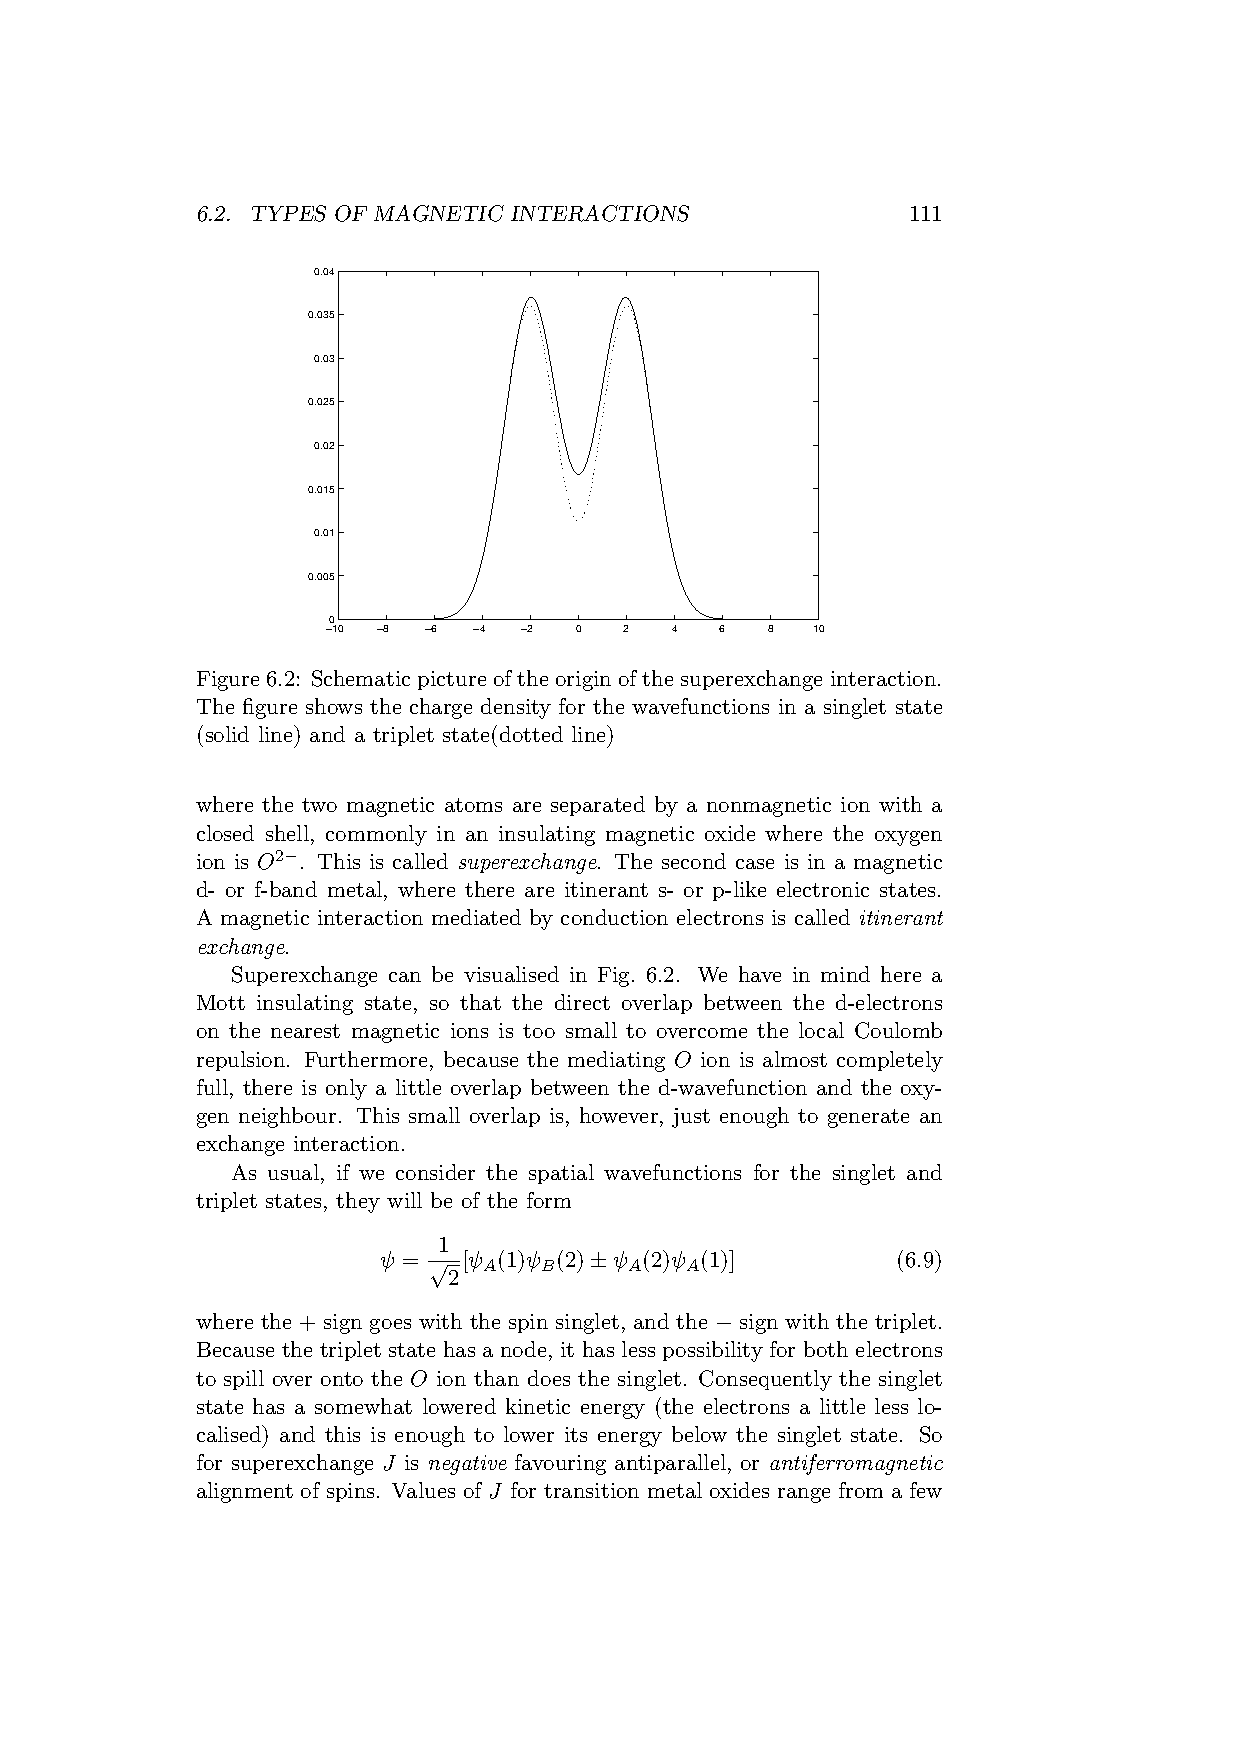
\includegraphics[width=0.5\textwidth,trim=5cm 19cm 7cm 4.5cm,clip]{6-2}
		\caption{[Figure~6.2 of the lecture notes] Charge density for the wavefunctions in a singlet state~(solid line) and a triplet state~(dotted line).}
		\label{f1}
	\end{figure}
}